\documentclass[12pt, a4paper, oneside]{ctexart}
\usepackage{pgfplots}
\pgfplotsset{compat=1.15}
\usepackage{mathrsfs}
\usetikzlibrary{arrows}
\usepackage{amsmath, amsthm, amssymb, appendix, bm, graphicx, hyperref, mathrsfs}
\usepackage{mathrsfs,esint,wrapfig,color,xcolor}
\title{\textbf{论文标题}}
\author{Dylaaan}
\date{\today}
\linespread{1.5}
\newtheorem{theorem}{定理}[section]
\newtheorem{definition}[theorem]{定义}
\newtheorem{lemma}[theorem]{引理}
\newtheorem{corollary}[theorem]{推论}
\newtheorem{example}[theorem]{例}
\newtheorem{proposition}[theorem]{命题}
\renewcommand{\abstractname}{\Large\textbf{摘要}}
\def\D{\mathrm{d}}
%\def\F{\ensuremath{f(z)}}
\def\Fex{\ensuremath{u(x,y)+iv(x,y)}}
\def\de{\ensuremath{\Delta}}
\newcommand{\partdev}[3][]
{\ensuremath{\frac{\displaystyle \partial^{#1} #2}{ \displaystyle \partial #3}}}
\newcommand{\F}[1][z]
{\ensuremath{f(#1)}}
\newcommand{\dev}[3][]
{\ensuremath{\frac{\displaystyle \D^{#1} #2}{ \displaystyle \D #3}}}
\begin{document}

\maketitle

\setcounter{page}{0}
\maketitle
\thispagestyle{empty}

\newpage
\pagenumbering{Roman}
\setcounter{page}{1}
\tableofcontents
\newpage
\setcounter{page}{1}
\pagenumbering{arabic}

\section{泰勒展开与劳伦展开的区别}

\subsection{泰勒级数和劳伦级数的定义}

泰勒展开的定义:

$\F$在$z_0$为圆心的圆域内解析,则对于任意一圆域内点$z$,有
\begin{align*}
    f & (z)=\sum_{n=0}^\infty a_n(z-z_0)^n                                                                 \\
    a & _n=\frac{1}{2\pi i}\ointctrclockwise \frac{\F[\xi]}{(\xi-z_0)^{n+1}}\D \xi=\frac{f^{(n)}(z_0)}{n!}
\end{align*}
\begin{proof}
    \begin{align*}
        \F & =\frac{1}{2\pi i}\ointctrclockwise_C \frac{\F[\xi]}{\xi-z}\D \xi=\frac{1}{2\pi i}\ointctrclockwise_C \frac{\F[\xi]}{(\xi-z_0)-(z-z_0)}\D \xi \\
           & =\frac{1}{2\pi i}\ointctrclockwise_C \frac{\F[\xi]}{\xi-z_0}\frac{1}{1-\frac{z-z_0}{\xi-z_0}}\D \xi
    \end{align*}
    由于


    \begin{equation}
        \label{spanseries}
        \color{red}
        \frac{z-z_0}{\xi-z_0}\le 1,\quad\frac{1}{1-t}=\sum_{n=0}^\infty t^n,\;\; |t|<1
    \end{equation}

    \begin{align*}
         & \frac{1}{2\pi i}\ointctrclockwise_C \frac{\F[\xi]}{\xi-z_0}\frac{1}{1-\frac{z-z_0}{\xi-z_0}}\D \xi                       \\
         & =\frac{1}{2\pi i}\ointctrclockwise_C \frac{\F[\xi]}{\xi-z_0}\sum_{n=0}^\infty \left[\frac{z-z_0}{\xi-z_0}\right]^n\D \xi \\
         & =\sum_{n=0}^\infty \left[\frac{1}{2\pi i}\ointctrclockwise_C \frac{\F[\xi]}{(\xi-z_0)^{n+1}}\D \xi\right](z-z_0)^n=\F
    \end{align*}
\end{proof}
复变函数在其解析圆域上的泰勒级数展开的收敛半径为:
$$
    R=\lim_{n\to \infty}\frac{1}{\sqrt[n]{|a_n|}}=\lim_{n\to \infty} \left| \frac{a_n}{a_{n+1}} \right| \;\; or \;\; R=|z_0-z_1| \;\; \text{$z_1$是离$z_0$最近的奇点}
$$

劳伦展开的定义:

$\F$在以$z_0$为圆心的环域内解析,则对于该环域内任何一点$z$,有
\begin{align*}
     & \F = \sum_{n=-\infty}^\infty                                                                 \\
     & a_n (z-z_0)^n\quad\quad a_n=\frac{1}{2\pi i} \ointctrclockwise \F[\xi](\xi-z_0)^{-n-1}\D \xi
\end{align*}
\begin{proof}
    将环域的外环和内环建立一微小链接,使得$L=C_1+C_2+\partial L - \partial L = C_1+C_2$为一单连通区域的边界,
    \begin{align*}
        \F = \frac{1}{2\pi i} \ointctrclockwise_L \frac{\F[\xi]}{\xi-z}\D \xi=\frac{1}{2\pi i} \ointctrclockwise_{C_1} \frac{\F[\xi]}{\xi-z}\D \xi+\frac{1}{2\pi i} \ointclockwise_{C_2} \frac{\F[\xi]}{\xi-z}\D \xi \\
        = \frac{1}{2\pi i} \ointctrclockwise_{C_1} \frac{\F[\xi]}{\xi-z}\D \xi -\frac{1}{2\pi i} \ointctrclockwise_{C_2} \frac{\F[\xi]}{\xi-z}\D \xi                                                                 \\
    \end{align*}
    回想起证明泰勒级数时的过程,不妨将$\xi-z_0$设为$r$,$z-z_0$设为$R$,不难发现:对于$C_1$,$r>R$,对于$C_2$,$r<R$。
    \begin{align*}
        \frac{1}{2\pi i} \ointctrclockwise_{C_1} \frac{\F[\xi]}{\xi-z}\D \xi
         & = \frac{1}{2\pi i} \ointctrclockwise_{C_1} \frac{\F[\xi]}{r-R}\D \xi                                                              \\
         & = \frac{1}{2\pi i} \ointctrclockwise_{C_1} \frac{\F[\xi]}{1-R/r}\D \xi                                                            \\
         & =\frac{1}{2\pi i} \ointctrclockwise_{C_1} \sum_{n=0}^\infty \left(\frac{R}{r}\right)^n  \frac{\F[\xi]}{\xi-z_0} \D \xi            \\
         & =\frac{1}{2\pi i} \ointctrclockwise_{C_1} \sum_{n=0}^\infty  \left(\frac{z-z_0}{\xi-z_0}\right)^n  \frac{\F[\xi]}{\xi-z_0} \D \xi
    \end{align*}
    同理可得
    \begin{align*}
        -\frac{1}{2\pi i} \ointctrclockwise_{C_2} \frac{\F[\xi]}{\xi-z}\D \xi
         & = -\frac{1}{2\pi i} \ointctrclockwise_{C_2} \frac{\F[\xi]}{r-R}\D \xi                                                           \\
         & = \frac{1}{2\pi i} \ointctrclockwise_{C_2} \frac{\F[\xi]}{1-r/R}\D \xi                                                          \\
         & =\frac{1}{2\pi i} \sum_{n=0}^\infty \ointctrclockwise_{C_2} \left(\frac{r}{R}\right)^n  \frac{\F[\xi]}{z-z_0} \D \xi            \\
         & = \frac{1}{2\pi i} \ointctrclockwise_{C_2} \sum_{n=0}^\infty \left(\frac{\xi-z_0}{z-z_0}\right)^n  \frac{\F[\xi]}{z-z_0} \D \xi
    \end{align*}
    代入$\F$中得到
    \begin{align*}
        \F & =\frac{1}{2\pi i} \ointctrclockwise_{C_1} \sum_{n=0}^\infty  \left(\frac{z-z_0}{\xi-z_0}\right)^n  \frac{\F[\xi]}{\xi-z_0} \D \xi
        + \frac{1}{2\pi i} \ointctrclockwise_{C_2} \sum_{n=0}^\infty \left(\frac{\xi-z_0}{z-z_0}\right)^n  \frac{\F[\xi]}{z-z_0} \D \xi        \\
           & = \frac{1}{2\pi i}  \sum_{n=0}^\infty \left[\ointctrclockwise \frac{\F[\xi]}{(\xi-z_0)^{n+1}}\D \xi \right](z-z_0)^n              \\
           & +\frac{1}{2\pi i}  \sum_{n=-\infty}^{-1} \left[\ointctrclockwise \frac{\F[\xi]}{(\xi-z_0)^{n+1}}\D \xi\right](z-z_0)^n            \\
           & = \frac{1}{2\pi i}  \sum_{n=-\infty}^\infty \left[\ointctrclockwise \frac{\F[\xi]}{(\xi-z_0)^{n+1}}\D \xi \right](z-z_0)^n
    \end{align*}
\end{proof}
劳伦级数的收敛半径:
$$
    R_1<|z-z_0|<R_2,\quad R_1=\lim_{n\to -\infty} \left| \frac{a_{n-1}}{a_n} \right|\quad R_2=\lim_{n \to \infty} \left| \frac{a_n}{a_{n+1}} \right|
$$
或者可以认为
$$R_1 := \text{以$z_0$为圆心的包含考察点$z$的最大解析环域的内径}$$
$$R_2 := \text{以$z_0$为圆心的包含考察点$z$的最大解析环域的外径}$$

泰勒展开的使用范围是:对于某一在复平面上,以$z_0$为圆心的圆域内部均解析,才可以使用泰勒展开得到其相应的泰勒级数。如果不解析,会发生什么情况呢?
我们尝试对$f(z)=\frac{1}{z}$在$z_0=0$处进行泰勒展开,会发现由于泰勒展开的证明过程中使用到了柯西积分公式,使得$f$不适用。

柯西积分公式:假设$C$包围了$\F$的单连通解析区域,$z_0$为区域内一点,则
$$\F[z_0]=\frac{1}{2\pi i}\ointctrclockwise_C \frac{\F}{z-z_0}\D z$$

考虑到函数解析的定义,$f$在$z_0=0$处不解析等价为
$$
    \left. f'(z) \right|_{z=0} \text{不存在}
$$

\subsection{适用范围的差异}

考虑到柯西积分公式的证明过程:
不妨用一个小圆将$z_0=0$包围,其边界设为$\displaystyle C_r: \;\;\forall \; z\in \Sigma_{C_r}\quad z=+re^{i\theta}$,则由柯西积分定理,
\begin{align*}
    \ointctrclockwise_C \frac{\F}{z}\D z =\ointctrclockwise_{C_r}\frac{\F}{z}\D z =\int_0^{2\pi}{\color{red}\frac{\F[re^{i\theta}]}{re^{i\theta}}}ire^{i\theta}\D \theta
\end{align*}
{\color{red} 红色}部分会在接下来的证明过程中(令$r\to 0$)导出错误,因为
$$
    \lim_{r\to 0} \frac{\F[re^{i\theta}]}{re^{i\theta}} = \lim_{z\to 0} \frac{f(z)}{z} \;\; \text{不存在}
$$
这也是为什么泰勒展开仅仅适用于在圆域内全解析的情况。

而劳伦展开,通过构建合适的积分路径可以避免以上情况的发生,因此劳伦级数也可以适用于当$f(z)$在$z_0$处不解析的区域。例如:对于$f(z)=1/z$,通过将泰勒展开式
$$
    f(z)=\sum_{n=0}^\infty a_n(z-0)^n=\sum_{n=0}^\infty a_n z^n
$$
中的$z^n$替换为$\displaystyle(\frac{1}{z})^n$,使得原式的$f(z)$变为$f(1/z)$。

\subsection{表达式的差异}

考虑泰勒级数的系数表达式:
$$
    a_n=\frac{1}{2\pi i}\ointctrclockwise_{C_1} \frac{\F[\xi]}{(\xi-z_0)^{n+1}}\D \xi=\frac{f^{(n)}(z_0)}{n!}\;\;\; \text{For $n\ge 0$}
$$
其中$C_1$是任一解析圆域内部可求长的包围住了$z_0$的闭合曲线。

以及劳伦级数的系数表达式:
$$
    a_n=\frac{1}{2\pi i}\ointctrclockwise_{C_2} \frac{\F[\xi]}{(\xi-z_0)^{n+1}}\D \xi \;\;\; \text{For $-\infty \le n\le +\infty$}
$$
其中$C_2$是任一解析环域内部可求长的包围住了$z_0$的闭合曲线。

不难发现,当函数$f(z)$仅仅拥有可去奇点时($\forall \; n < 0, \;a_n=0$),其劳伦展开就是其泰勒展开。因为任一$C_2$,一定也是其$C_1$。同时,由于劳伦展开和泰勒展开的唯一性,
我们可以部分使用泰勒展开帮助计算劳伦展开。
\begin{example}
    对$f(z)=\displaystyle \frac{1}{z(z-1)}\quad |z|>1$进行劳伦展开。
    \begin{align*}
        &f(1/z)=\frac{z^2}{1-z}=z^2 \sum_{n=0}^\infty z^n = \sum_{n=2}^\infty z^n \qquad |z|<1 \\
        &f(z)=\sum_{n=2}^\infty z^{-n}=\sum_{n=-2}^\infty z^n \qquad |z|>1
    \end{align*}
\end{example}
\subsection{特殊点的差异}
一个函数如果以$z_0$为圆心的环域做劳伦展开,那么根据其劳伦展开的系数,$z_0$可以是$f(z)$的:
\begin{enumerate}
    \item 可去奇点,如果其展开不含负数项且包含常数项。
    \item $m-$阶零点,如果其最小的正数数项是$m$阶的。
    \item $m-$阶极点,如果其最小的负数项是$-m$阶的。
    \item 本性奇点,如果其展开包含无穷负数项。
\end{enumerate}
当$f(z)$在整个圆域内解析时,其劳伦展开就是其泰勒展开。且由于其解析性质,$z_0$不可能是$f(z)$的极点和本性奇点。换言之,泰勒展开不可能
拥有极点和本性奇点,只有可能拥有零点和可去奇点。而劳伦展开则可能拥有上述四种特殊点的的任一一种(不过显然$z_0$只会是四种特殊点中的其中一种)。

不妨假设$b$是$\F$的$m-$阶极点,那么:
$$
\begin{aligned}
f(z) &=a_{-m}(z-b)^{-m}+a_{-m+1}(z-b)^{-m+1}+\ldots+a_{0}+a_{1}(z-b)+\ldots \\
&=(z-b)^{-m}\left[a_{-m}+a_{-m+1}(z-b)+\ldots\right] \\
&=(z-b)^{-m} \phi(z), \quad 0<|z-b|<R
\end{aligned}
$$
则
$$
\frac{1}{f(z)}=(z-b)^{m} \frac{1}{\phi(z)}
$$
换言之,如果$z_0$是$\F$的$m$阶极点,那么$z_0$也是$1/\F$的$m$阶零点。

\section{复数域上根式函数和对数函数多值性的来源}
众所周知,复数域上的根式函数
$$
r_n(z)=\sqrt[n]{z}
$$
和对数函数
$$
L(z)=\operatorname{Ln}(z)
$$
拥有其在实数域上所不具备的多值性。下面我们对两个函数分别进行讨论。
\subsection{根式函数的多值性来源}
实数域中,根式函数定义为幂函数的反函数:
$$\forall\; x,y\in \mathbb{R}:\quad f(x)=y=x^n \to f^{-1}(y)=x=\sqrt[n]{y}$$
实数域中的根式函数有时也会遇到“多值性”。考虑函数$f(x)=x^2$,其反函数$f^{-1}(y)$似乎存在两个值对应。如图:

\begin{figure}[h]
    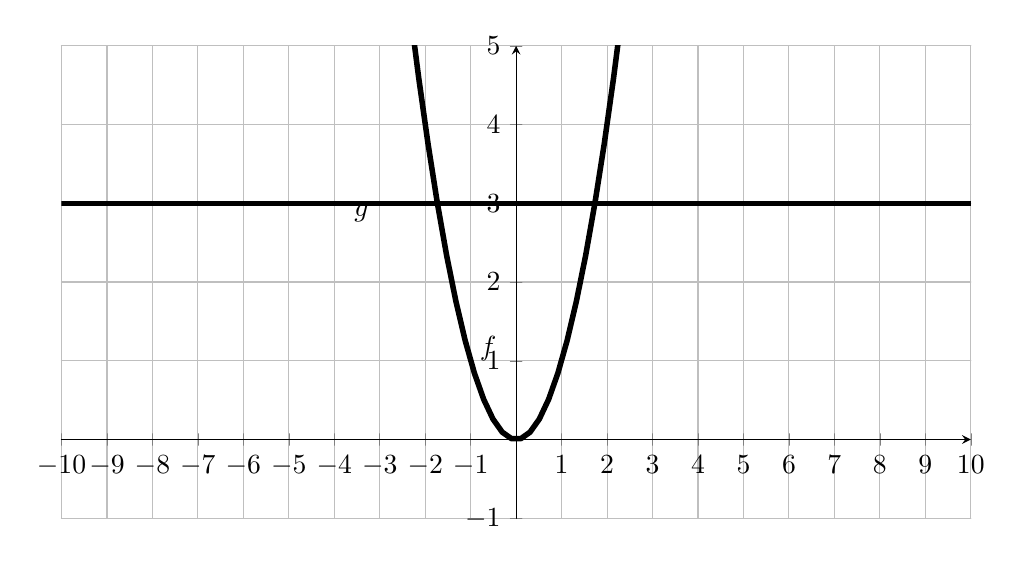
\begin{tikzpicture}[line cap=round,line join=round,>=triangle 45,x=\textwidth/22,y=1.0cm]
        \begin{axis}[
        x=\textwidth/21,y=1.0cm,
        axis lines=middle,
        ymajorgrids=true,
        xmajorgrids=true,
        xmin=-10.0,
        xmax=10.0,
        ymin=-1.0,
        ymax=5.0,
        xtick={-10.0,-9.0,...,10.0},
        ytick={-1.0,0.0,...,5.0},]
        \clip(-10.,-1.) rectangle (10.,5.);
        \draw [samples=50,rotate around={0.:(0.,0.)},xshift=0.cm,yshift=0.cm,line width=2.pt,domain=-5.0:5.0)] plot (\x,{(\x)^2/2/0.5});
        \draw [line width=2.pt,domain=-10.:10.] plot(\x,{(--3.-0.*\x)/1.});
        \begin{scriptsize}
        \draw[color=black] (-0.6143722943722925,1.1583549783549796) node {$f$};
        \draw[color=black] (-3.402251082251079,2.8726406926406947) node {$g$};
        \end{scriptsize}
        \end{axis}
        \end{tikzpicture}
\end{figure}

对于$f(x)=x^2$,任一一个给定的$y$都有两个$x$值与$y$对应,这意味着$y=x^2$的严格定义的反函数有可能具备某种多值性。然而,
为何实数域上,当我们定义其反函数时,只定义在了$y>0$的情况?

\begin{figure}[h]
    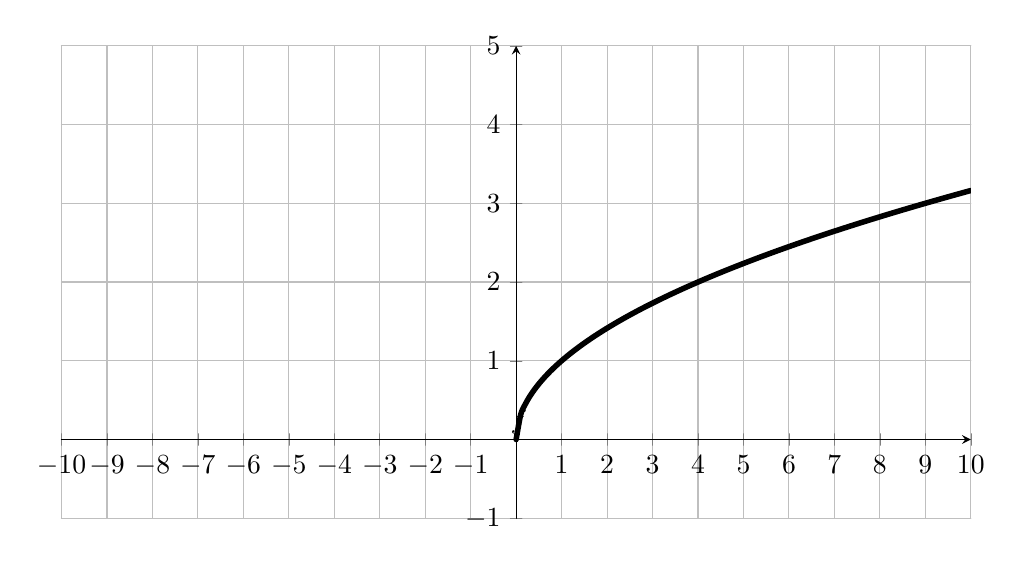
\begin{tikzpicture}[line cap=round,line join=round,>=triangle 45,x=\textwidth/22,y=1.0cm]
        \begin{axis}[
        x=\textwidth/21,y=1.0cm,
        axis lines=middle,
        ymajorgrids=true,
        xmajorgrids=true,
        xmin=-10.0,
        xmax=10.0,
        ymin=-1.0,
        ymax=5.0,
        xtick={-10.0,-9.0,...,10.0},
        ytick={-1.0,0.0,...,5.0},]
        \clip(-10.,-1.) rectangle (10.,5.);
        \draw[line width=2.pt,color=black,smooth,samples=100,domain=1.9999999794608742E-7:10.0] plot(\x,{sqrt((\x))});
        \begin{scriptsize}
        \draw[color=black] (0.05955663569354158,0.23335676720969983) node {$f$};
        \end{scriptsize}
        \end{axis}
    \end{tikzpicture}
\end{figure}
这可能是为了简化实数域内的相关计算。

由欧拉公式,在复数域内,
$$
e^{i\theta}=\cos \theta + i \sin \theta
$$
那么由三角函数的诱导公式,得到:
$$
e^{i\theta+2n\pi i}=\cos (\theta+2n\pi) + i \sin (\theta+2n\pi)=\cos \theta + i \sin \theta=e^{i\theta}
$$
考虑到任何一个复平面上的复数都可以表示为
$$
z=r\cdot e^{i\theta}=re^{i\theta+2n\pi i}
$$
假定$r=1$,那么根据幂运算的性质,根式函数$r_k(z)$:
$$
\sqrt[k]{z}=e^{(i\theta+2n\pi i)/k}=e^{i\theta/k+2n\pi i/k} =e^{i\theta/k+\Sigma}
$$
其中$\Sigma$:
$$
\Sigma = 2 \pi i /k + 4 \pi i/k+\dots+2(k-1)\pi i/k
$$
也就是说,如果我们约定$k\in \mathbb{Z}$, 那么一个$k$次方根式函数,拥有$k$个不同的多值分支。众所周知,一个复数$z$可以写成
$$
z=x+iy\;\; z\in\mathbb{C} \;\; x,y \in \mathbb{R}
$$
如果我们令$y=0$,则复数$z$“退化”为了实数。但是,根据复数根式函数的定义,当$y=0$时,其辐角$\theta=n\pi$,则
$$
z=e^{in\pi}
$$
那么根式函数(以二次根为例)
$$
r_2(z)=e^{in\pi/2}=e^{0i}\;\; \text{or} \;\; e^{i\pi}
$$
换言之,即使$z$“退化”为了实数,根式函数的多值性依然保留,而不是像实数域的根式函数一样只保留其中的一支,也意味着复数域上的根式函数与实数域上的根式函数有着本质区别,
复数域上的根式函数更“严格”地保留了幂函数反函数的意义。

\subsection{对数函数的多值性的来源}
实数域中,(自然)对数函数定义为指数函数的反函数:
$$\forall\; x,y\in \mathbb{R}:\quad f(x)=y=e^x \to f^{-1}(y)=x=\ln y$$
与实数域的根式函数不同,实数域的指数函数是不存在多值性的。

\begin{figure}[h]
    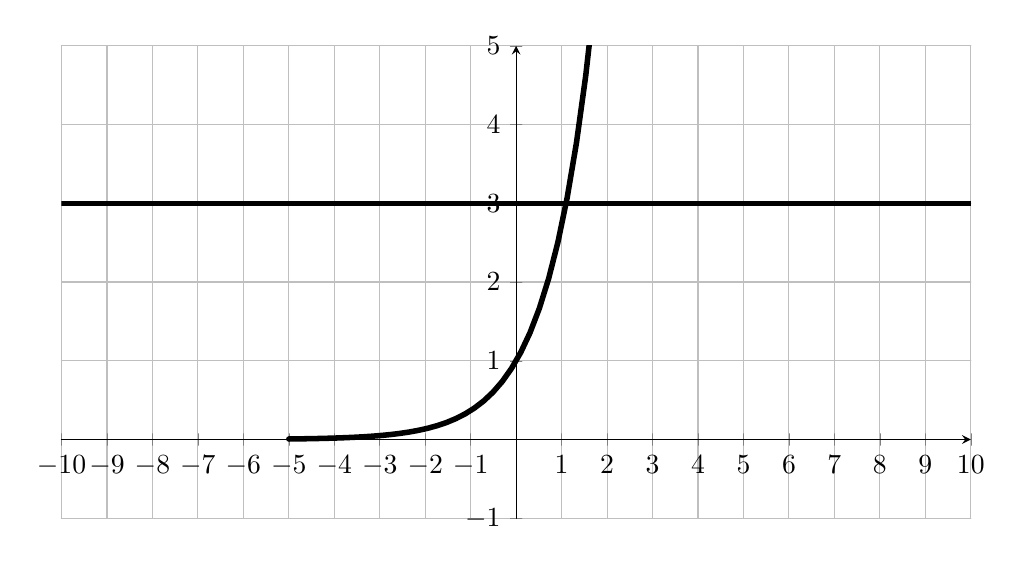
\begin{tikzpicture}[line cap=round,line join=round,>=triangle 45,x=\textwidth/22,y=1.0cm]
        \begin{axis}[
        x=\textwidth/21,y=1.0cm,
        axis lines=middle,
        ymajorgrids=true,
        xmajorgrids=true,
        xmin=-10.0,
        xmax=10.0,
        ymin=-1.0,
        ymax=5.0,
        xtick={-10.0,-9.0,...,10.0},
        ytick={-1.0,0.0,...,5.0},]
        \clip(-10.,-1.) rectangle (10.,5.);
        \draw [samples=50,rotate around={0.:(0.,0.)},xshift=0.cm,yshift=0.cm,line width=2.pt,domain=-5.0:5.0)] plot (\x,{(e^\x)/2/0.5});
        \draw [line width=2.pt,domain=-10.:10.] plot(\x,{(--3.-0.*\x)/1.});
        \begin{scriptsize}
        \end{scriptsize}
        \end{axis}
        \end{tikzpicture}
\end{figure}

由欧拉公式,在复数域内,
$$
e^{i\theta}=\cos \theta + i \sin \theta
$$
那么由三角函数的诱导公式,得到:
$$
e^{i\theta+2n\pi i}=\cos (\theta+2n\pi) + i \sin (\theta+2n\pi)=\cos \theta + i \sin \theta=e^{i\theta}
$$
考虑到任何一个复平面上的复数都可以表示为
$$
z=r\cdot e^{i\theta}=re^{i\theta+2n\pi i}
$$
那么根据幂运算的性质,对数函数$\operatorname{Ln} z$:
$$
\operatorname{Ln} z = \operatorname{Ln} r  e^{i\theta} = \operatorname{Ln} r e^{i\theta + 2n\pi i} = \ln r + i(\theta+2n\pi i) = \ln |z| + i(\theta+2n\pi i)
$$
注意到,当$z$“退化”为实数时,其辐角
\begin{align*}
    \theta = 
    \begin{cases}
        2n\pi\quad x > 0\\
        \pi+2n\pi \quad x\le 0
    \end{cases}
\end{align*}
如果我们在实数域约定$\theta \in [0,2\pi)$,则复数域$\operatorname{Ln} z$
\begin{align*}
    \theta = 
    \begin{cases}
        0\quad x > 0\\
        \pi \quad x\le 0
    \end{cases}
\end{align*}
由于实数域中的指数函数恒大于0,则指数函数不可能包含$\theta=\pi$的分支,也就退化为了实数域的自然对数函数。换言之,复数域中指数函数的多值性的根本来源为
将原定义域为实数域的对数函数拓展至复数域的过程中。同根式函数一样,复数域的对数函数与实数域的根式函数也存在根本差异。当$z$退化为实数时,对其使用复数域的指数函数,其结果也不等于
实数域的对数函数。
\section{复数与实数、复函数与实函数的区别}
实数与复数、实数函数和复数函数的区别有许多。接下来我们分别讨论。
\subsection{实数与复数的区别}
实数与复数的最主要区别是,复数相比实数增加了一个基元(base) $i$,并且让其具备了所有实数都不具备的性质:
$$
i^2=-1
$$
通过两种基$1$与$i$的任意线性组合,可以表示任一复数和实数。

同时,不同于实数域可以排序,复数域是无法排序的。也就是说,不存在某种关系,我们定义为“$>$”、“$<$”以及“$=$”:
设 $a, b, c \in \mathbb{C}$ 是复数,
\begin{enumerate}
    \item 对于$a$和$b$,要么$a > b$,要么$a < b$,要么$a = b$
    \item 如果 $a < b$ ,那么 $a+c < b+c$ 。
    \item 如果 $a < b$ 并且 $c>0$ ,那么 $a c < b c$ 。
    \item 如果 $a < b$ 并且 $c<0$ ,那么 $a c > b c$ 。
\end{enumerate}
下面我们举一个反例:假设$i>0$,则由上条性质2,
$$
i\cdot i > i \cdot 0 \Leftrightarrow -1 > 0
$$
显然矛盾。若$i<0$,则由上条性质3,
$$
i \cdot i > 0 \cdot i \Leftrightarrow -1 >0
$$
显然矛盾,且显然$i\ne 0$。这说明如果引入了$i$,便无法再定义一个关系满足以上四种性质。
\subsection{复变函数和实变函数的区别}
一元实变函数与复变函数的最本质区别是,复变函数是某种特殊的“二元函数”,因为任一一个复数$z$都可以表示成:
$$
z=x+iy
$$
这样的形式。也即:
$$
\text{复函数}f: \mathbb{C} \rightarrow \mathbb{C}
$$
$$
\text{一元实函数}f: \mathbb{R}^1 \rightarrow \mathbb{R}^1
$$
$$
\text{二元实函数}f: \mathbb{R}^2 \rightarrow \mathbb{R}^2
$$
而因此,当我们在讨论复变函数的“可导”与“可微”时,这两个概念便不会像一元实变函数那样等价。但是,如果$f(z)$可以直接写成$z$的形式(而不是实部虚部分离的形式),
复变函数又表现出了一元实函数的部分特性,看上去像是一个一元函数。

而能否认为复变函数是特殊的二元实变函数呢?考虑到二元函数连续的定义:

\begin{equation*}
    \lim _{\substack{x \rightarrow x_{0} \\ y \rightarrow y_{0}}} f(x, y)=A
\end{equation*}


注意到二元实函数连续要求以任何方向$(x,y)\to(x_0,y_0)$时其极限均存在且相等。复变函数$u(z)$可以写成
$$
u(z)=u(x,y)=v(z)+iw(z)=v(x,y)+iw(x,y) \quad x,y,v,w \in \mathbb{R}
$$
形式如上的复变函数的连续性等价为$u$和$w$均连续。也就是说,只要一个复变函数的实部和虚部分别连续,那么这个复变函数一定连续;反之,无法从二元实变函数中找到类似的两个部分,使得当这两个部分分别连续时,实变函数一定连续。

考虑到二元实变函数的可微定义:
$$
z=f(x,y)\;\; \text{可微} \Leftrightarrow \D z = A \D x + B \D y
$$
而二元实变函数即使在$x$和$y$方向均可导,也不意味着其可微。例如:
\begin{example}
\begin{align*}
f(x, y)=\begin{cases}\displaystyle
\frac{x y}{ \sqrt{x^{2}+y^{2}}}\quad  (x, y) \neq(0,0) \\
0 \quad (x, y)=(0,0)
\end{cases} 
\end{align*}
\begin{equation*}
    \lim _{x \rightarrow 0} \frac{f(x, 0)-f(0,0)}{x-0}=\lim _{x \rightarrow 0}\left(\frac{\displaystyle \frac{0}{|x|}-0}{x}\right)=0 \Rightarrow f_{x}^{\prime}(0,0)=0
\end{equation*}
同理,$f'_y(0,0)=0$。但是,其微分:
\begin{equation*}
    \begin{aligned}
    &\Delta z=f(0+\Delta x, 0+\Delta y)-f(0,0)=\frac{\Delta x \cdot \Delta y}{\sqrt{(\Delta x)^{2}+(\Delta y)^{2}}} \\
    &\text { 直接带入 } \frac{x y}{\sqrt{x^{2}+y^{2}}} \text { 得到 } \\
    &A=0, \quad B=0, \rho=\sqrt{(\Delta x)^{2}+(\Delta y)^{2}} \\
    &\lim _{\rho \rightarrow 0} \frac{\Delta z}{\rho}=\lim _{\substack{\Delta x \rightarrow 0 \\
    \Delta y \rightarrow 0}} \frac{\sqrt{(\Delta x)^{2}+(\Delta y)^{2}}}{\sqrt{(\Delta x)^{2}+(\Delta y)^{2}}}=\lim _{\substack{\Delta x \rightarrow 0 \\
    \Delta y \rightarrow 0}} \frac{\Delta x \cdot \Delta y}{(\Delta x)^{2}+(\Delta y)^{2}} \\
    & \lim _{\Delta x \rightarrow 0} \frac{\Delta x \cdot \Delta y}{(\Delta x)^{2}+(\Delta y)^{2}}=\frac{1}{2} ; \lim _{\substack{x \rightarrow 00 \\
    \Delta y=-\Delta x}} \frac{\Delta x \cdot \Delta y}{(\Delta x)^{2}+(\Delta y)^{2}}=-\frac{1}{2}
    \end{aligned}
\end{equation*}
\end{example}
说明$f(x,y)$的微分不存在。说明$f(x,y)$在$x$、$y$方向上的偏导不一定能完全表示其微分性质,即使保证了
$$
f_x(x,y)=f_y(x,y)
$$
也无法保证在沿着其他方向求得的偏导相等,进而也无法保证其导数存在。换言之,函数$f(x,y)$的偏导数存在,也不一定可微。仅仅当偏导数存在且连续时,其可微。

而复变函数,似乎很少谈论其“偏导数”。复变函数$u(z)$写成
$$
u(z)=u(x,y)=v(z)+iw(z)=v(x,y)+iw(x,y) \quad x,y,v,w \in \mathbb{R}
$$
即使$u$的实部和虚部的偏导数均存在且连续,也无法认为其在区域内可微。还需要考虑Cauchy-Riemann条件:
$$
\left\{
\begin{aligned}
    \frac{\displaystyle \partial u(x,y)}{ \displaystyle \partial x}=\frac{\displaystyle \partial v(x,y)}{\displaystyle \partial y} \\
    \frac{\displaystyle \partial v(x,y)}{ \displaystyle \partial x}=-\frac{\displaystyle \partial u(x,y)}{\displaystyle \partial y}
\end{aligned}
\right.
$$

除此之外,复变函数的“解析性”带来的一些性质也是复变函数所独有的。考虑二元实变函数所类似的性质“区域内可微”。一个解析函数所具有的零点是孤立的。而区域内可微的实变函数,其零点未必是孤立的。例如函数:
\begin{equation*}
    f(x)=\left\{\begin{array}{l}
    x^{2} \sin \frac{1}{x}, x \neq 0 \\
    0, x=0
    \end{array}\right.
\end{equation*}

同时,由于复数可以表示成以下形式:
$$
z=re^{i\theta}
$$
所以复变函数还具有实变函数所不具备的柯西积分公式、留数定理等数学工具。

不过,实变函数也具备一些复变函数所不具备的性质。例如Lagrange中值定理:
比如设 $f(z)=z^{3}+1, z_{1}=\frac{-1+\sqrt{3} i}{2}, z_{2}=\frac{-1-\sqrt{3} i}{2}$, 则有 $f\left(z_{2}\right)-f\left(z_{1}\right)=0$, $z_{2}-z_{1}=-\sqrt{3} i$, 显然连接 $z_{1}$ 和 $z_{2}$ 
的线段上的任意一点 $x$, 都不可能使得等式 $f\left(z_{2}\right)-f\left(z_{1}\right)=f^{\prime}(\xi)\left(z_{2}-z_{1}\right)$ 成立, 即 Lagrange 中值定理不成立.
\end{document}